%\chapter{Results}

%\section{Problem A: Pathfinding in 2D Games}

All deliverables in the form of code are enclosed.

\subsection*{Subproblem A.1: Grids with Obstacles}

The following figures show the solution path calculated by the A* implementation,
with the $\text{OPEN}$ and $\text{CLOSED}$ sets visualized as respectively cyan
and pink dots.

\begin{figure}[h!]
  \centering
    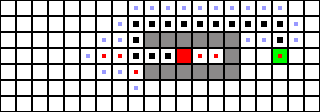
\includegraphics[width=0.8\textwidth]{img/board-1-1-astar}
    \caption{Board 1.1}
\end{figure}

\begin{figure}[h!]
  \centering
    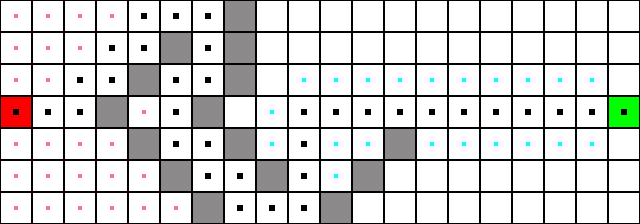
\includegraphics[width=0.8\textwidth]{img/board-1-2-astar}
    \caption{Board 1.2}
\end{figure}

\begin{figure}[h!]
  \centering
    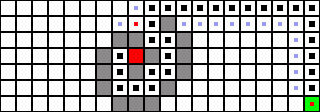
\includegraphics[width=0.8\textwidth]{img/board-1-3-astar}
    \caption{Board 1.3}
\end{figure}

\begin{figure}[h!]
  \centering
    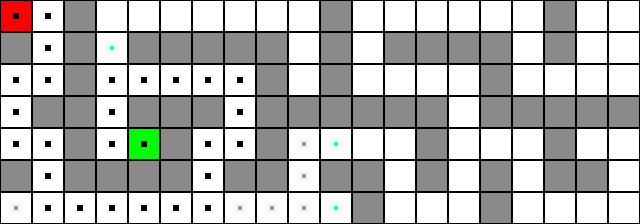
\includegraphics[width=0.8\textwidth]{img/board-1-4-astar}
    \caption{Board 1.4}
\end{figure}

\clearpage

\subsection*{Subproblem A.2: Grids with different cell costs}

For this subproblem, we modified our implementation to be able to parse weighted
boards as well as correctly handling cost calculation of weighted nodes.
Again, the visualizations include the $\text{OPEN}$ and $\text{CLOSED}$ sets.

\begin{figure}[h!]
  \centering
    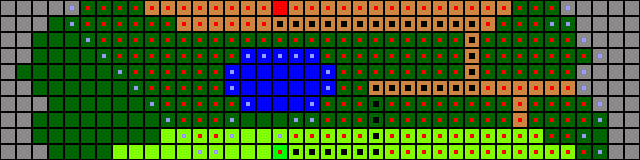
\includegraphics[width=\textwidth]{img/board-2-1-astar}
    \caption{Board 2.1}
\end{figure}

\begin{figure}[h!]
  \centering
    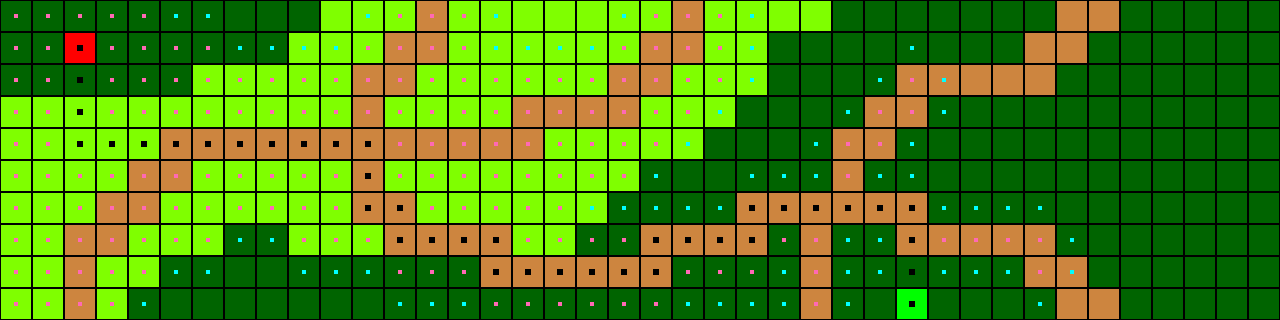
\includegraphics[width=\textwidth]{img/board-2-2-astar}
    \caption{Board 2.2}
\end{figure}

\begin{figure}[h!]
  \centering
    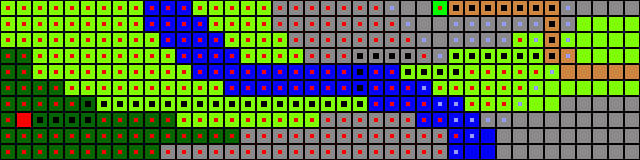
\includegraphics[width=\textwidth]{img/board-2-3-astar}
    \caption{Board 2.3}
\end{figure}

\begin{figure}[h!]
  \centering
    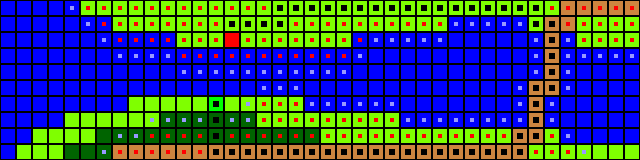
\includegraphics[width=\textwidth]{img/board-2-4-astar}
    \caption{Board 2.4}
\end{figure}

\clearpage

\subsection*{Comparison with BFS and Dijkstra's Algorithm}

\subsubsection*{Board 1.1}

\begin{figure}[h!]
  \centering
    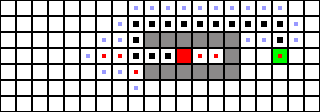
\includegraphics[width=0.8\textwidth]{img/board-1-1-astar}
    \caption{Board 1.1 - A*}
\end{figure}

\begin{figure}[h!]
  \centering
    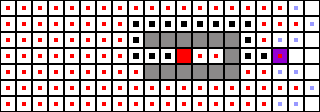
\includegraphics[width=0.8\textwidth]{img/board-1-1-dijkstra}
    \caption{Board 1.1 - Dijkstra}
\end{figure}

\begin{figure}[h!]
  \centering
    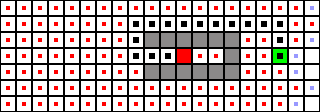
\includegraphics[width=0.8\textwidth]{img/board-1-1-bfs}
    \caption{Board 1.1 - BFS}
\end{figure}

All three algorithms find an equally short path, but A* examines significantly
fewer nodes doing it.

\clearpage

\subsubsection*{Board 1.2}

\begin{figure}[h!]
  \centering
    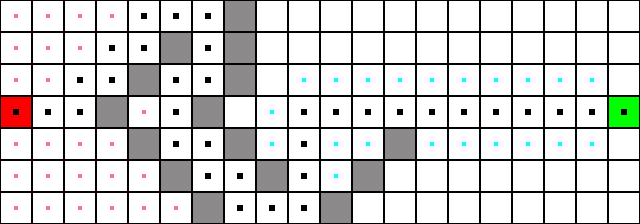
\includegraphics[width=0.8\textwidth]{img/board-1-2-astar}
    \caption{Board 1.2 - A*}
\end{figure}

\begin{figure}[h!]
  \centering
    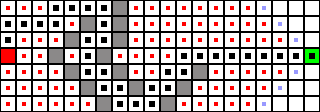
\includegraphics[width=0.8\textwidth]{img/board-1-2-dijkstra}
    \caption{Board 1.2 - Dijkstra}
\end{figure}

\begin{figure}[h!]
  \centering
    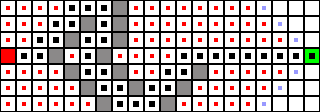
\includegraphics[width=0.8\textwidth]{img/board-1-2-bfs}
    \caption{Board 1.2 - BFS}
\end{figure}

All algorithms find the shortest path, but again, A* is much more efficient.

\clearpage

\subsubsection*{Board 1.3}

\begin{figure}[h!]
  \centering
    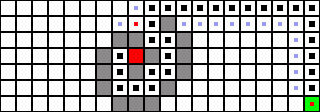
\includegraphics[width=0.8\textwidth]{img/board-1-3-astar}
    \caption{Board 1.3 - A*}

\end{figure}

\begin{figure}[h!]
  \centering
    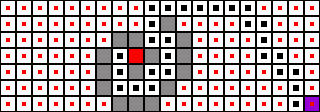
\includegraphics[width=0.8\textwidth]{img/board-1-3-dijkstra}
    \caption{Board 1.3 - Dijkstra}
\end{figure}

\begin{figure}[h!]
  \centering
    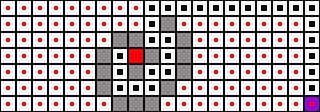
\includegraphics[width=0.8\textwidth]{img/board-1-3-bfs}
    \caption{Board 1.3 - BFS}
\end{figure}

Again, A* is much more efficient than the others.

\clearpage

\subsubsection*{Board 1.4}

\begin{figure}[h!]
  \centering
    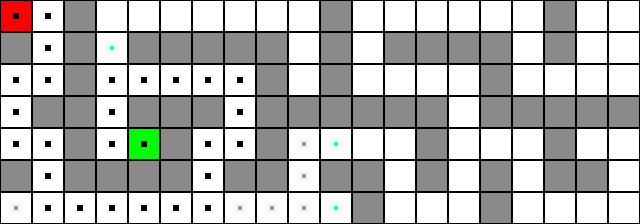
\includegraphics[width=0.8\textwidth]{img/board-1-4-astar}
    \caption{Board 1.4 - A*}
\end{figure}

\begin{figure}[h!]
  \centering
    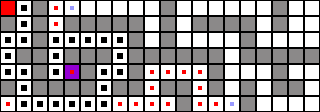
\includegraphics[width=0.8\textwidth]{img/board-1-4-dijkstra}
    \caption{Board 1.4 - Dijkstra}
\end{figure}

\begin{figure}[h!]
  \centering
    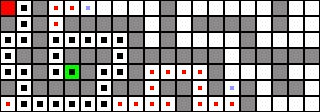
\includegraphics[width=0.8\textwidth]{img/board-1-4-bfs}
    \caption{Board 1.4 - BFS}
\end{figure}

For this board, we see that there's not much difference between the three
algorithms. A* explores marginally fewer nodes than the other two.

\clearpage

\subsubsection*{Board 2.1}

\begin{figure}[h!]
  \centering
    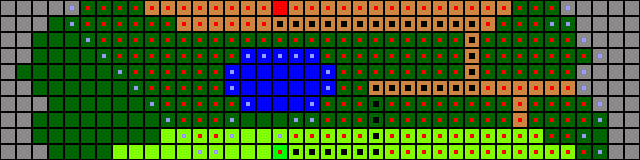
\includegraphics[width=\textwidth]{img/board-2-1-astar}
    \caption{Board 2.1 - A*}
\end{figure}

\begin{figure}[h!]
  \centering
    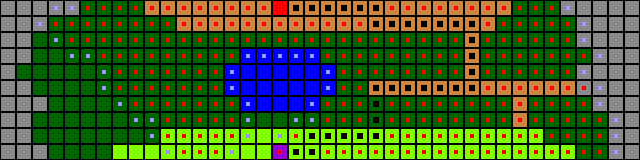
\includegraphics[width=\textwidth]{img/board-2-1-dijkstra}
    \caption{Board 2.1 - Dijkstra}
\end{figure}

\begin{figure}[h!]
  \centering
    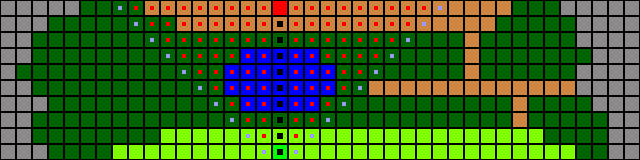
\includegraphics[width=\textwidth]{img/board-2-1-bfs}
    \caption{Board 2.1 - BFS}
\end{figure}

For this board, we see that A* and Djikstra both find equally optimal paths,
both processing about the same number of nodes. (A* slightly lower as the 
heuristic is taken into consideration.) BFS processes fewer nodes, but finds an
extremely unoptimized path.

\clearpage

\subsubsection*{Board 2.2}

\begin{figure}[h!]
  \centering
    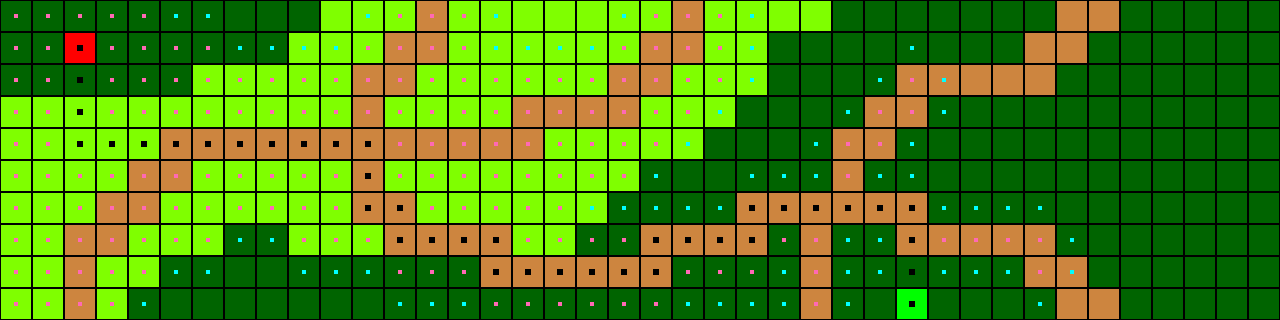
\includegraphics[width=\textwidth]{img/board-2-2-astar}
    \caption{Board 2.2 - A*}
\end{figure}

\begin{figure}[h!]
  \centering
    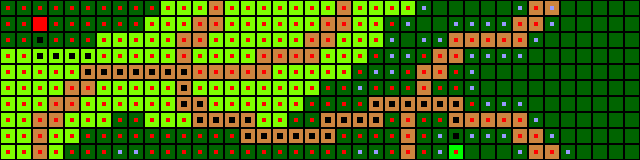
\includegraphics[width=\textwidth]{img/board-2-2-dijkstra}
    \caption{Board 2.2 - Dijkstra}
\end{figure}

\begin{figure}[h!]
  \centering
    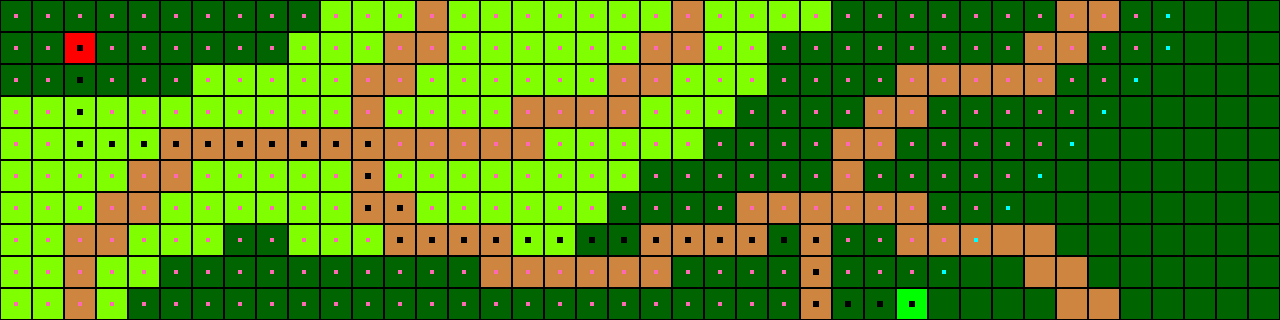
\includegraphics[width=\textwidth]{img/board-2-2-bfs}
    \caption{Board 2.2 - BFS}
\end{figure}

A* and Dijkstra both perform reasonably well here, while BFS makes quite a few
suboptimal choices while also processing more nodes.

For the case of A* vs. Djikstra, we see that A* (as it should) refrains from
processing nodes that have low cell weight, but also have higher heuristic values.

\clearpage

\subsubsection*{Board 2.3}

\begin{figure}[h!]
  \centering
    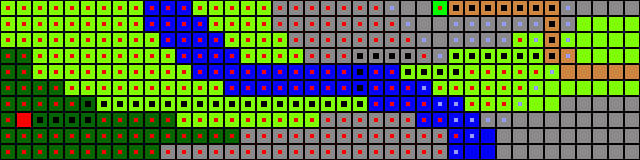
\includegraphics[width=\textwidth]{img/board-2-3-astar}
    \caption{Board 2.3 - A*}
\end{figure}

\begin{figure}[h!]
  \centering
    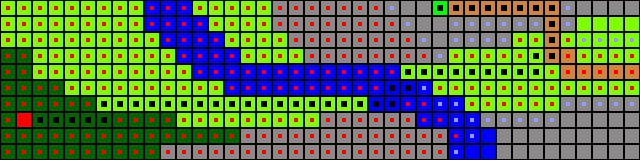
\includegraphics[width=\textwidth]{img/board-2-3-dijkstra}
    \caption{Board 2.3 - Dijkstra}
\end{figure}

\begin{figure}[h!]
  \centering
    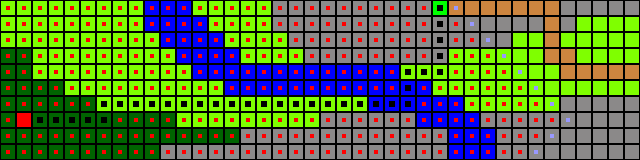
\includegraphics[width=\textwidth]{img/board-2-3-bfs}
    \caption{Board 2.3 - BFS}
\end{figure}

Again, A* and Dijkstra both find equally optimal paths, while BFS naively picks
the first path it can find.

\clearpage

\subsubsection*{Board 2.4}

\begin{figure}[h!]
  \centering
    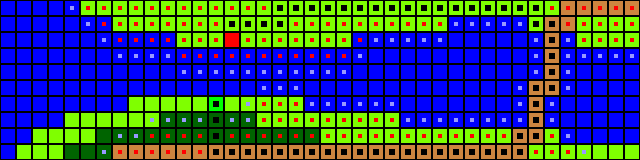
\includegraphics[width=\textwidth]{img/board-2-4-astar}
    \caption{Board 2.4 - A*}
\end{figure}

\begin{figure}[h!]
  \centering
    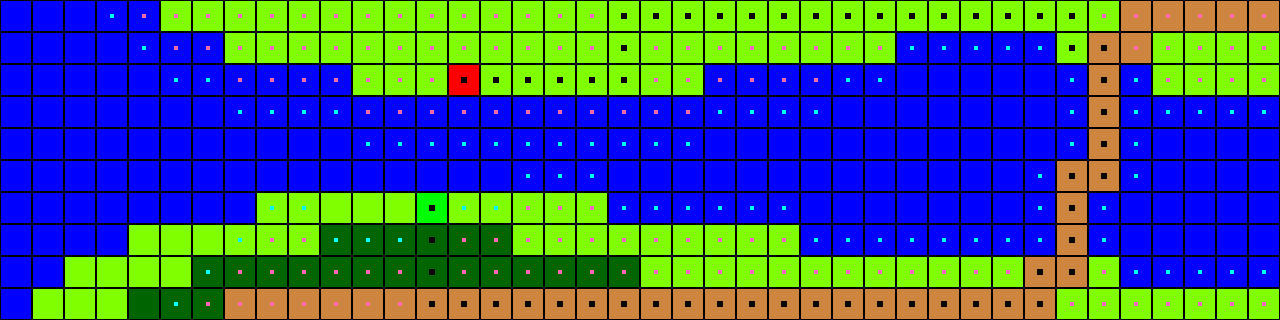
\includegraphics[width=\textwidth]{img/board-2-4-dijkstra}
    \caption{Board 2.4 - Dijkstra}
\end{figure}

\begin{figure}[h!]
  \centering
    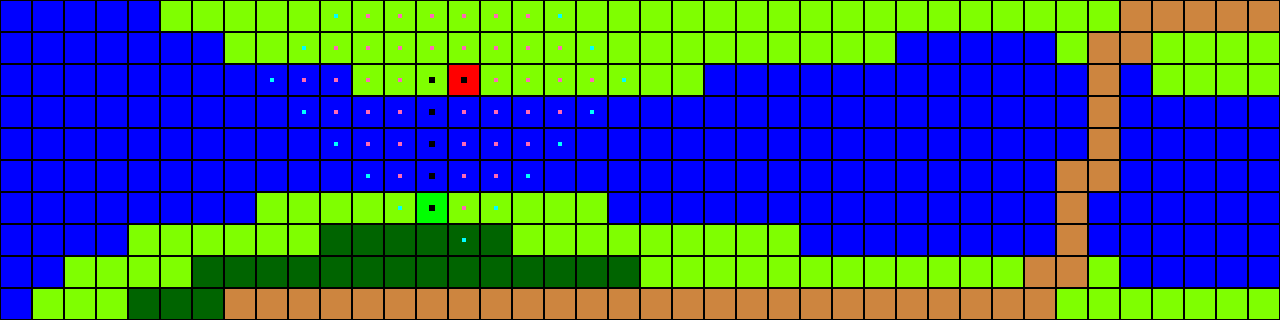
\includegraphics[width=\textwidth]{img/board-2-4-bfs}
    \caption{Board 2.4 - BFS}
\end{figure}

For this final board, A* and Dijkstra find the same path. A* processes slightly
fewer nodes, notably those in the bottom right corner of the board.
BFS processes few nodes, but finds a suboptimal path.


\begin{enumerate}

    \item
        The Turing test is determinines if an AI has a human-like intelligence. A human tester has a conversation, but whether the tester is talking to an AI or another human is not known to the tester. If an AI is able to convince the tester that it is human, the AI passes the Turing test.

    \item
        Thinking rationally is using reasoning and logic. Acting rationally is using rational thinking to decide on an action.

        A rational action can be taken without a corresponding rational thinking process, such as in the example of a reflexive recoil when touching a hot stove. No time is spent deliberating, another system takes immediate action.

    \item
        The theory explains how to relate abstract logical to the real world. Real world actions can thus be rationalized by more abstract logic.

    \item
        Performing a task by trying to increase performance AND decrease cost (increasing the performance/cost ratio). Requires that these are somehow quantifiable.

        "A rational agent chooses whichever action maximizes the expected value of the performance measure given the percept sequence to date."

    \item
        \begin{enumerate}[(a)]
            \item
                Assuming the robot has used the observation methods in it's action portfolio first, and made the decision to cross the road based on what it observed, the robot has acted rationally.
                Since the helicopter crash cannot be predicted by the robot based on it's observations, we cannot put any 'blame' on it and claim it acted irrationally.

            \item
                In this case the car should be within the observational range of the robot. However, the green light is also observable, and the robot would rightfully assume that the car (another agent) would follow the rules of the traffic light.
                Thus, the action of crossing the road on a green light seems rational.

        \end{enumerate}
    \item
        \begin{enumerate}[(a)]
            \item
                The simple reflex agent cannot be rational in this case because it doesn't track state in any way, such as whether it has already visited a tile. Thus it would go left and right over and over and lose many points.

            \item
                The reflex agent with state can be rational, as it can evaluate the first tile and clean if neccesary, then move to the other one and clean it if neccesary, then know it is done and not lose any more points.

            \item
                If the simple reflex agent can detect the state of the tiles in entire "universe" it operates in, then it can act rationally, because it can have a stop condition. See code in listing.
                \begin{figure}
                    \begin{lstlisting}[caption=Algorithm (python-like), language=Python, label=algo]
                    while (A_is_dirty or B_is_dirty):
                        if location == A:
                            if A_is_dirty:
                                suck()

                            if B_is_dirty:
                                right()
                        else:
                            if B_is_dirty:
                                suck()

                            if A_is_dirty:
                                left()
                    \end{lstlisting}
                \end{figure}
        \end{enumerate}

    \newpage
    \item
        \begin{itemize}
            \item   Partially observable. Because the robot can only sense the tile it is in.
            \item   Single agent. There is only the robot acting on the environment.
            \item   Deterministic. The cleaning operation will always succeed if it is started.
            \item   Episodic. The robot bases it's decision only on the current tile's state.
            \item   Static. The tile will not change while the robot is deliberating.
            \item   Discrete. The tiles are separate and there is no "in between".
            \item   Known. The robot knows that the tiles only have two possible states.
        \end{itemize}
    \item
        \begin{enumerate}[(a)]
            \item   Simple reflex agents
                \begin{itemize}
                    \item   Easier to implement.
                    \item   Not very intelligent, can easily get stuck in infinite loops.
                \end{itemize}
            \item   Model-based reflex agents
                \begin{itemize}
                    \item   Can avoid many of the problems of simple reflex agents by remembering state and reaching an end condition.
                \end{itemize}
            \item   Goal-based agents
                \begin{itemize}
                    \item   More flexible.
                    \item   Can have the concept of a compound goal and track the progress towards achieving this.
                    \item   Can consider multiple solutions to the problem and naïvely pick the best.
                \end{itemize}
            \item   Utility-based agents
                \begin{itemize}
                    \item   Good in environments where optimization is possible.
                    \item   Can consider multiple solutions, their costs, and pick the one which solves the problem for the lowest cost.
                \end{itemize}
        \end{enumerate}
\end{enumerate}
